\documentclass[%
    BCOR=8.25mm,         % Bindekorrektur
    DIV=11,              % Satzspiegel
    openany,
    parskip=half,        % Abstand zwischen Absätzen
    bibliography=totoc,  % Literaturverzeichnis im Inhaltsverzeichnis
    headsepline=on,      % Trennlinie Kolumnentitel
]{scrbook}

% Préambule
\usepackage[a4paper, top=2cm, bottom=2cm, left=2cm, right=2cm]{geometry}
\usepackage[ngerman]{babel} % Deutsche typogr. Regeln + Trenntabelle
\usepackage[T1]{fontenc}             % TeX Font-Codierung
\usepackage{lmodern}                 % Latin Modern font
\usepackage[utf8]{inputenc}          % Font-Codierung der Eingabedatei
\usepackage[babel]{csquotes}         % Anführungszeichen
\usepackage{graphicx} % Graphiken
\usepackage{here}  % Neu eingefügt
\usepackage{caption}                 % Bildunterschrift
\usepackage{booktabs}                % Tabellen schöner
\usepackage{listingsutf8}            % Listings mit Einstellungen
\usepackage{amsmath}	               % Mathematik
\usepackage[pdftex]{hyperref}  
\usepackage{xurl} % Erlaubt URL-Umbrüche
\hypersetup{
    bookmarksopen=true,
    bookmarksopenlevel=3,
    colorlinks,
    citecolor=blue,
    linkcolor=blue,
}
\usepackage{scrhack}  % Unterdrückt Fehlermeldung von listings
\usepackage{microtype}
\usepackage{tabularx}
\usepackage{hyperref}
\usepackage{fancyhdr}
\pagestyle{fancy}

% Clear headers and footers to customize
\fancyhf{} 

% Customize the footer
\fancyfoot[C]{
    
\includegraphics[width=6cm]{img/mni-logo.pdf} % Adjust the logo size here
    \hspace{0.4cm} % Adjust the space between logo and text
    Danielou Mounsande Sandamoun\hspace{0.7cm} \thepage
} 

\renewcommand{\headrulewidth}{0pt} 
\renewcommand{\footrulewidth}{0.4pt} 




% Configuration du Stil für die Bibliographie
\usepackage[
    backend=biber,       % Verwende Biber als Backend
    backref,             % Rückverweise von Literatur ins Dokument
    style=numeric,       % Numerischer Zitierstil
    sorting=none,         % Sortierung nach Name, Jahr, Titel
    isbn=false           % ISBN in der Bibliographie ausblenden
]{biblatex}

% Lade die Citavi-Bibliothek
\addbibresource{zitationen.bib} % Name der .bib-Datei

%% Numérotation des sections und Tiefe des Inhalts
\setcounter{tocdepth}{3}             % 3 Stufen im Inhaltsverzeichnis
\setcounter{secnumdepth}{3} 		     % 3 Stufen in Abschnittnummerierung

% ----------------------------------------------------------------------------
\begin{document}
%% Titelseite
\begin{titlepage}
    \begin{center}
    
\includegraphics[width=0.9\textwidth]{img/mni-logo.pdf}\\[4cm]
    
    \textbf{\huge\sffamily Einsatz von künstlicher Intelligenz in eingebetteten Systemen
    }\\[1.5cm]
    \Large Wissenschaftliche Arbeit\\
    Ingenieur-Informatik Bachelor of Science (B.Sc.)
    \\[1cm]
    Vorgelegt von\\ [1.0cm]
    
    Danielou Mounsande Sandamoun\\~\\
    Februar 2025
    \end{center}
    \vfill
    \begin{tabular}{ll}
        Referent der Arbeit: & Niklas Philipp\\ 
    \end{tabular}
\end{titlepage}
\cleardoubleemptypage

%% Sperrvermerk
\newpage

\cleardoubleemptypage

%% Verzeichnisse
\tableofcontents
%\listoffigures
%\listoftables
%\lstlistoflistings

\mainmatter 
\pagestyle{fancy}

% Beispiel für eine Zitation
\chapter{Einleitung}
Die zunehmende Integration von Machine Learning in eingebettete Systeme wird durch mehrere Schlüsselfaktoren motiviert. Ein zentraler Aspekt ist die Fähigkeit von Machine Learning, die Leistung und Funktionalität solcher Systeme erheblich zu verbessern. Eingebettete Systeme, die oft in ressourcenbeschränkten Umgebungen arbeiten, profitieren von der Effizienz und Entscheidungsfähigkeit, die Machine Learning bietet. Beispielsweise ermöglichen fortschrittliche Algorithmen und maschinelles Lernen eine präzise Verarbeitung und Analyse von Sensordaten in Echtzeit, was für Anwendungen im Gesundheitswesen, der Automobilindustrie und in industriellen Umgebungen von entscheidender Bedeutung ist \cite{Gembaczka.2019}.\\
Im Gesundheitswesen können eingebettete ML-Systeme eine Echtzeit-Überwachung und -Analyse von Vitaldaten ermöglichen \cite{Gembaczka.2019}, was zu einer verbesserten Patientenüberwachung und -versorgung führt. In der Automobilindustrie unterstützen Machine-Learning-gesteuerte eingebettete Systeme fortschrittliche Fahrerassistenzsysteme (ADAS) und autonomes Fahren, indem sie Umgebungsdaten verarbeiten und schnelle Entscheidungen treffen. Industrie 4.0 profitiert von Machine Learning in eingebetteten Systemen durch die Optimierung von Produktionsprozessen und die vorausschauende Wartung von Maschinen, was zu einer höheren Effizienz und geringeren Ausfallzeiten führt \cite{Gembaczka.2019}.\\
Das Ziel dieser Arbeit besteht darin, einen umfassenden Einblick in die Nutzung von Machine Learning in eingebetteten Systemen zu gewähren. Es werden sowohl die grundlegenden Konzepte als auch deren Anwendungsbereiche beschrieben. Ein besonderer Schwerpunkt liegt auf der Integration von Machine Learning in eingebettete Systeme, wobei die Vorteile, Herausforderungen und praktischen Implementierungsbeispiele analysiert werden. Ziel ist es, ein tieferes Verständnis für die Potenziale und Grenzen von Machine Learning in diesem Kontext zu schaffen und mögliche zukünftige Forschungsrichtungen aufzuzeigen.
\chapter{Grundlagen}
\section{Einführung in eingebettete Systeme}
\subsection{Definition}
Eingebettete Systeme sind informationsverarbeitende Systeme, die in umgebende Produkte integriert sind \cite {Marwedel.2021}. Sie sind aus unserem Alltag nicht mehr wegzudenken und bilden die Grundlage moderner Technologien. Je nach Schwerpunkt ergibt sich eine leicht unterschiedliche Definition:  
\begin{itemize}
    \item Marwedel definiert eingebettete Systeme als \glqq informationsverarbeitende Systeme, die in umgebende Produkte integriert sind.\grqq\cite{Marwedel.2021}.
    \item In der englischen Literatur wird der Fokus auf die Software gelegt: \glqq Embedded software is software integrated with physical processes. The technical problem is managing time and concurrency in computational systems.\grqq\cite{Marwedel.2021}.
    \item Die dritte Definition betont die Interaktion mit der Umgebung: \glqq Cyber-physikalische Systeme (engl. Cyber-Physical Systems (CPS)) bestehen aus der Integration von Berechnungen und physikalischen Prozessen.\grqq\cite{Marwedel.2021}.
\end{itemize}  

Die verschiedenen Definitionen zeigen, dass eingebettete Systeme nicht nur aus Hardware bestehen, sondern auch eine enge Verzahnung mit Software und physikalischen Prozessen aufweisen.  

\subsection{Eingebettete Systeme und Cyber-physikalische Systeme (CPS)}
Ein Cyber-physikalisches System (CPS) kann als eine Weiterentwicklung eingebetteter Systeme betrachtet werden. Während eingebettete Computersysteme den Fokus auf die informationsverarbeitende Einheit legen, erweitert ein CPS diesen Ansatz durch die Integration von Netzwerken und Echtzeit-Interaktionen mit der Umgebung \cite{Marwedel.2021}.  

Die folgende Abbildung \ref{fig:cbs-systeme} visualisiert die Architektur eines CPS. Solche Systeme kombinieren eingebettete Computersysteme mit Netzwerken, um physikalische Prozesse zu steuern und Daten in Echtzeit auszutauschen. Dies macht sie zu einem zentralen Element der Industrie 4.0 \cite{Westermann.2016}.  
CPS ermöglichen intelligente, vernetzte und automatisierte Systeme, die in vielen Branchen – von der Automobilindustrie bis zur Medizintechnik – eingesetzt werden \cite{Westermann.2016}. Eingebettete Systeme, eingebettete Computersysteme und CPS sind somit eng miteinander verbunden, wobei CPS die umfassendste Form darstellen.  

\begin{figure}[h]
	\centering
	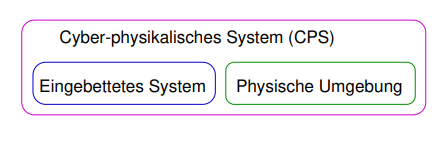
\includegraphics[width=0.9\textwidth]{img/CPS.png}
	\caption{Abbildung zu CPS \cite{Marwedel.2021}}
	\label{fig:cbs-systeme}
\end{figure}
Die Definitionen eingebetteter Systeme können zu Beginn für den Leser schwer verständlich sein. Daher wird im Folgenden eine zusätzliche Erklärung zu eingebetteten Systemen gegeben.  

Historisch war die Informationsverarbeitung eng mit Großrechnern und großen Bandlaufwerken verbunden. Die Miniaturisierung der Technologie führte jedoch zur Einführung von Personal Computern (PCs), die zunächst primär für Büroanwendungen eingesetzt wurden \cite{Ubiquitous_Computing_1994}. Parallel dazu entstanden Rechner, die speziell für Steuerungs- und Regelungsaufgaben in physischen Systemen konzipiert wurden \cite{Ubiquitous_Computing_1994}.  

Mark Weiser prägte später den Begriff des „allgegenwärtigen Rechnens“ (ubiquitous computing). Er prognostizierte, dass Computer und Informationen zukünftig jederzeit und überall verfügbar sein würden und dass Computer so in Produkte integriert würden, dass sie für den Nutzer unsichtbar sind \cite{Ubiquitous_Computing_1994}. Diese Entwicklung führte zur Einführung des Konzepts des „unsichtbaren Computers“. Beispiele hierfür sind unter anderem Fernbedienungen, Kameras oder Mobiltelefone.  

Verwandte Konzepte sind das \textbf{durchdringende Rechnen} (pervasive computing) und die \textbf{umgebende Intelligenz} (ambient intelligence). Diese Begriffe betonen unterschiedliche Aspekte der modernen Informationstechnologie:  
\begin{itemize}
    \item \textbf{Allgegenwärtiges Rechnen}: Ziel ist es, Informationen jederzeit und überall bereitzustellen \cite{Ubiquitous_Computing_1994}.  
    \item \textbf{Durchdringendes Rechnen}: Fokussiert sich auf die praktische Anwendung und Nutzung vorhandener Technologien \cite{Ubiquitous_Computing_1994}.  
    \item \textbf{Umgebende Intelligenz}: Bezieht sich auf die Nutzung von Informationstechnologie, beispielsweise in intelligenten Wohnhäusern oder Bürogebäuden \cite{Ubiquitous_Computing_1994}.
\end{itemize}  

Viele dieser Konzepte sind mittlerweile Realität geworden, insbesondere durch die Verbreitung kleiner mobiler Geräte und des mobilen Internets, das zahlreiche Bereiche des täglichen Lebens beeinflusst. Darüber hinaus wird die Künstliche Intelligenz künftig eine zentrale Rolle in der Weiterentwicklung dieser Technologien spielen. Auf diesen Aspekt wird später eingegangen.  

Ein weiterer wesentlicher Bestandteil eingebetteter Systeme ist der Kommunikationsaspekt. Abbildung \ref{fig:kommunikation} illustriert die Beziehung zwischen Kommunikation und eingebetteten Systemen.  
\begin{figure}[h]
	\centering
	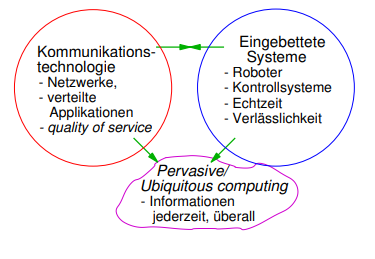
\includegraphics[width=0.9\textwidth]{img/kommunikation.png}
	\caption{Kommunikation und eingebettete Systeme \cite{Marwedel.2021}}
	\label{fig:kommunikation}
\end{figure}
Die "National Science Foundation" (NSF) in den USA hebt die Bedeutung der Vernetzung und Kommunikation verteilter Systeme im Kontext Cyber-physikalischer Systeme (CPS) hervor. In deutscher Übersetzung wird festgestellt, dass diese aufkommenden Systeme „koordiniert, verteilt und verbunden sein werden und dass sie robust und reaktionsfähig sein müssen“ \cite{Council.2015}.  

Cyber-physikalische Systeme stellen eine Weiterentwicklung eingebetteter Systeme  dar. Während eingebettete Systeme meist isoliert und spezialisiert für spezifische Aufgaben entwickelt werden, zeichnen sich CPS durch ihre umfassende Vernetzung und die Integration physischer und digitaler Prozesse aus \cite{Marwedel.2021}. Eingebettete Systeme agieren hauptsächlich lokal und reaktiv, ohne größere Datenanalysen oder Interaktionen mit anderen Systemen durchzuführen \cite{Marwedel.2021}. CPS hingegen sind proaktiv, verteilt und in der Lage, Daten in Echtzeit zu verarbeiten und Entscheidungen zu treffen, um komplexe und dynamische Aufgaben zu bewältigen \cite{Marwedel.2021}. Diese Eigenschaften machen CPS zu einem unverzichtbaren Bestandteil moderner Anwendungen, die zunehmend auf Vernetzung und Automatisierung angewiesen sind.  

Diese Aussage verdeutlicht die Anforderungen an moderne CPS, die nahtlose Kommunikation und Kooperation gewährleisten müssen, selbst wenn sie über unterschiedliche geografische Standorte verteilt sind. Solche Systeme müssen nicht nur zuverlässig (robust) arbeiten, sondern auch in der Lage sein, auf Veränderungen in ihrer Umgebung schnell und flexibel zu reagieren \cite{Council.2015}.  

Diese Eigenschaften sind essenziell für die erfolgreiche Integration von CPS in verschiedenen Anwendungsbereichen, wie etwa in der Automobilelektronik, der Robotik, intelligenten Gebäuden, dem Gesundheitswesen, der Agrartechnik, der öffentlichen Sicherheit oder dem Maschinenbau \cite{Westermann.2016, Council.2015, Wang.2021}.


\section{Einführung in künstliche Intelligenz}

Künstliche Intelligenz ist ein Forschungsfeld, das auf der Nachbildung menschlicher kognitiver Fähigkeiten basiert \cite{Amit.2018, Koricanac.2021, Zhang.2023}. Eine geeignete Analogie, um KI zu erklären, ist das menschliche Gehirn. Dieses besteht aus etwa 85 Milliarden Nervenzellen, sogenannten Neuronen, die kontinuierlich elektrische Impulse erzeugen \cite{Amit.2018}. Jedes Neuron bildet zehntausende Verbindungen zu seinen Nachbarzellen \cite{Amit.2018}. Dieses hochkomplexe System ist die Grundlage für Lernprozesse, Schlussfolgerungen und abstraktes Denken.  

Die zentrale Frage lautet: Ist es möglich, ein solches System künstlich nachzubilden? Was genau ist künstliche Intelligenz?  

\subsection{Definition und Kategorien der künstlichen Intelligenz}

Künstliche Intelligenz basiert im Wesentlichen auf Algorithmen, also Computerprogrammen \cite{Amit.2018, Koricanac.2021, Zhang.2023}. Dabei wird KI in drei Hauptkategorien unterteilt:

1. \textbf{Schwache KI}:  
   Schwache KI ist auf spezifische Aufgabenbereiche spezialisiert\cite{Funk.2022}. viele alltägliche Anwendungen, wie Sprachassistenten (z. B. Siri) oder Spamfilter in E-Mails, basieren auf schwacher KI. Diese Systeme sind sehr leistungsfähig in ihrem jeweiligen Bereich, können ihre Erkenntnisse jedoch nicht auf andere Domänen übertragen.

2. \textbf{Starke KI}:  
   Starke KI beschreibt Systeme, die über ähnliche kognitive Fähigkeiten wie der Mensch verfügen \cite{Funk.2022}. Im Gegensatz zur schwachen KI wäre eine starke KI in der Lage, Schlussfolgerungen von einem Bereich auf andere zu übertragen \cite{Funk.2022}.

3. \textbf{Künstliche Superintelligenz}:  
   Die künstliche Superintelligenz beschreibt hypothetische Systeme, die in allen Aspekten menschliche Intelligenz übertreffen könnten \cite{Funk.2022}.

\subsection{Von schwacher KI zu starker KI}

Ein zentraler Forschungsbereich der KI ist die Frage, wie schwache KI-Systeme in starke KI überführt werden können. Ein Ansatz hierbei ist die Nachahmung des menschlichen Lernprozesses durch künstliche neuronale Netze \cite{Funk.2022}.

Künstliche neuronale Netze bestehen aus miteinander verbundenen künstlichen Neuronen, die in mehreren Schichten organisiert sind \cite{Lammel.2023}. Während der Trainingsphase erhält das Netzwerk große Mengen an Daten. Das Netzwerk lernt durch Rückmeldungen, ob ein Bild korrekt erkannt wurde oder nicht. Das Netzwerk lernt durch Rückmeldungen, ob ein Bild korrekt erkannt wurde oder nicht. Auf dieser Basis werden die Verbindungen zwischen den Neuronen angepasst: Verbindungen, die zu korrekten Ergebnissen führen, werden verstärkt, während Verbindungen, die zu fehlerhaften Ergebnissen führen, geschwächt werden \cite{Lammel.2023}.

Nach zahlreichen Trainingszyklen entwickelt sich das Netzwerk zu einem sogenannten intelligenten neuronalen Netzwerk, das sich selbst optimieren kann. Dieser Prozess wird als \emph{Deep Learning} bezeichnet \cite{Lammel.2023}. Deep Learning hat bereits zahlreiche Bereiche revolutioniert, darunter Bildverarbeitung, Spracherkennung und autonome Systeme \cite{Lammel.2023}.

\chapter {Nutzung von Künstlicher Intelligenz auf eingebettete Systeme
}

\section{Anwendung, Beispiele zur erfolgreichen Implementierung von KI in eingebetteten 
Systemen}
\subsection{Spezielles Beispiel: Autonome Fahrzeuge}
Im Folgenden wird die Interaktion zwischen dem eingebetteten System und der KI am Beispiel eines autonomen Fahrzeugs näher erläutert.\\
Autonome Fahrzeuge, wie Autos und Busse, sind in der Lage, Hindernisse eigenständig zu erkennen und bei Bedarf anzuhalten. Diese Fähigkeit basiert auf einer Vielzahl von eingebetteten Systemen, die durch Künstliche Intelligenz  gesteuert werden. Wie in Abbildung \ref{fig:Kommu} dargestellt, verfügen autonome Fahrzeuge über eine komplexe Sensorik, darunter LIDAR, Radar, IMU (Inertiale Messeinheit), sowie Kameras und GPS-Antennen, die zusammenarbeiten, um Umgebungsdaten zu erfassen und zu analysieren.
\begin{figure}[h]
	\centering
	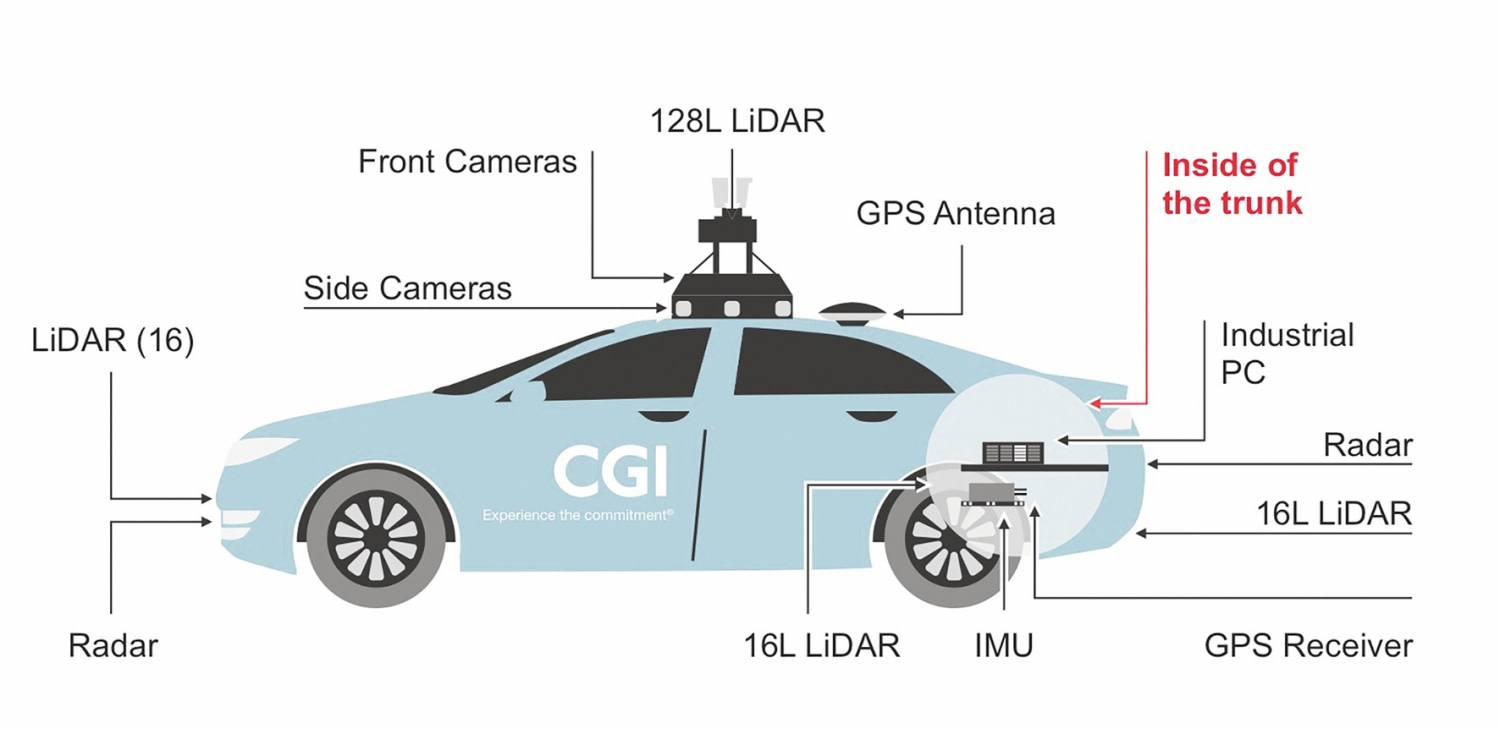
\includegraphics[width=0.9\textwidth]{img/Fahzeuge_GCI.jpg}
	\caption{Beispiel eines autonomen Fahrzeugs\textsuperscript{01}}
	\label{fig:Kommu}
\end{figure}
\footnotetext{\textsuperscript{1}Quelle: \url{https://www.hanser-automotive.de/a/fachartikel/besser-sein-als-der-mensch-211161}}

Die Abbildung \ref{fig:Kommu} zeigt die Architektur eines autonomen Fahrzeugs, bei dem mehrere Sensoren strategisch positioniert sind, um eine 360-Grad-Überwachung zu gewährleisten. Der LIDAR-Sensor spielt eine zentrale Rolle bei der Erstellung von präzisen 3D-Karten der Umgebung, während Radarsysteme die Erkennung von beweglichen Objekten wie anderen Fahrzeugen und Fußgängern unterstützen. Kameras sind unerlässlich für die visuelle Analyse von Verkehrszeichen, Straßenmarkierungen und Ampeln, was eine detaillierte Navigation ermöglicht. Die Kombination dieser Daten mit GPS-Positionierung sorgt für eine genaue Lokalisierung des Fahrzeugs auf digitalen Karten.\\
Durch diese Integration kann das Fahrzeug, wie in der Abbildung illustriert, Entscheidungen in Echtzeit treffen, zum Beispiel das Anhalten an Kreuzungen oder das Umfahren von Hindernissen. Hochleistungsrechner, wie sie in autonomen Fahrzeugen verwendet werden, ermöglichen die Verarbeitung der von den Sensoren gesammelten Daten und steuern das Fahrzeug entsprechend. Firmen wie Waymo und Tesla nutzen solche Architekturen, um die Sicherheit und Effizienz ihrer Systeme zu verbessern.\\
Die Abbildung verdeutlicht somit die wesentliche Rolle von eingebetteten KI-Systemen bei der Realisierung autonomer Fahrzeuge und dient als Beispiel für die erfolgreiche Integration von Sensorik, Aktorik und KI-gestützten Algorithmen.\\

\subsection{Weitere Beispiele von Anwendung von KI in eingebette Systeme}
Neben der Anwendung von KI in autonomen Fahrzeugen finden künstliche Intelligenz und eingebettete Systeme auch in zahlreichen anderen Bereichen vielfältige Einsatzmöglichkeiten. Ein Beispiel hierfür ist die "MindSphere"-Plattform von Siemens, eine offene IoT-Plattform, die in eingebetteten Systemen industrieller Anlagen integriert ist. Diese Plattform nutzt KI zur Analyse von Sensordaten von Maschinen, um potenzielle Ausfälle vorherzusagen und die Wartung zu optimieren. Durch den Einsatz von maschinellem Lernen kann das System kontinuierlich lernen und Anomalien in Produktionsprozessen frühzeitig erkennen, was die Effizienz und Zuverlässigkeit in der Industrie verbessert.\\
Auch im Bereich der Sicherheits- und Überwachungstechnik hat Hikvision Künstliche Intelligenz in seine eingebetteten Kamerasysteme integriert. Die abgebildete Kamera in Abbildung \ref{fig:hikvision} illustriert den Einsatz von KI-gestützter Überwachungstechnik, bei der fortschrittliche Bildverarbeitungsalgorithmen und maschinelles Lernen eine zentrale Rolle spielen. Die Systeme ermöglichen eine präzise Erkennung von Personen in Echtzeit sowie eine automatische Analyse von Verhaltensmustern. Dies erlaubt es, verdächtige Aktivitäten frühzeitig zu identifizieren und angemessen darauf zu reagieren.\\  

\begin{figure}[h]
	\centering
	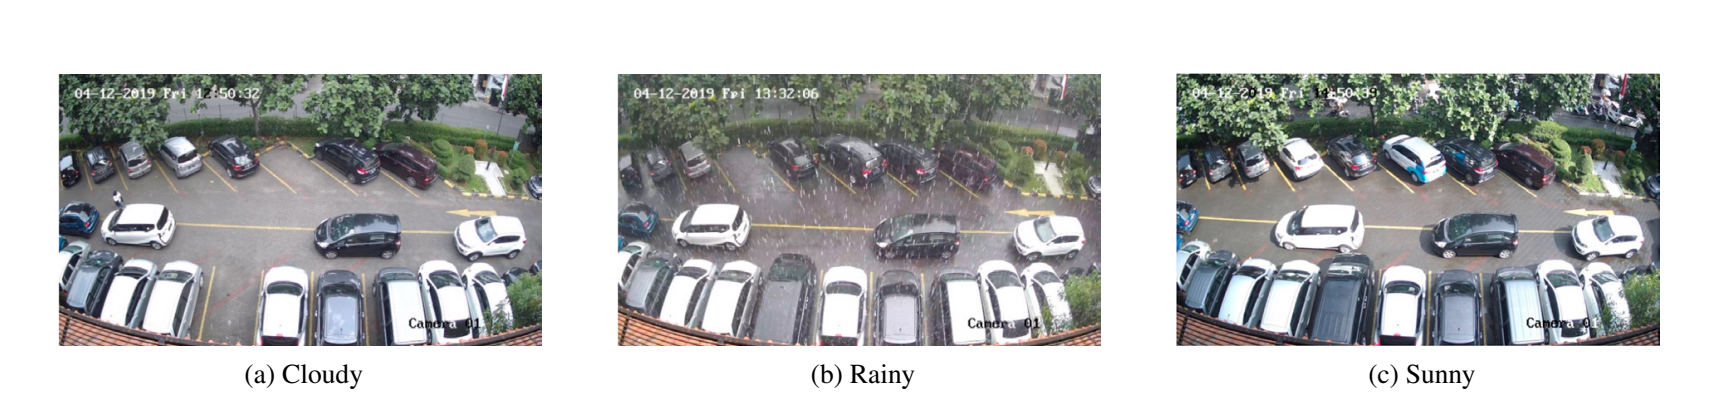
\includegraphics[width=0.9\textwidth]{img/hikvision_parking.png}
	\caption{Hikvision IP-Kamera zur Überwachung der Parkplatzbelegung \cite{Farley.2021}}
	\label{fig:hikvision}
\end{figure}  
Ein konkretes Anwendungsbeispiel für KI-gestützte Überwachungssysteme ist die automatische Erkennung von Parkraumbelegung. Die in Abbildung \ref{fig:hikvision} gezeigte Kamera nutzt Deep-Learning-Modelle wie AlexNet und mAlexNet, um in Echtzeit zwischen belegten und freien Parkplätzen zu unterscheiden. Die Forschungsergebnisse zeigen, dass diese Systeme eine Erkennungsgenauigkeit von bis zu 93,15 \% erreichen und eine Parkplatzanalyse innerhalb von 0,5 Sekunden pro Stellplatz durchführen können \cite{Farley.2021}.  

Durch den Einsatz dieser Technologie wird die Effizienz von Parkraummanagementsystemen erheblich gesteigert. Autofahrer können schneller freie Parkplätze finden, was nicht nur den Verkehrsfluss verbessert, sondern auch den Kraftstoffverbrauch und die Umweltbelastung reduziert. Die Integration von KI in solche Überwachungssysteme zeigt, wie maschinelles Lernen und eingebettete Systeme zur Optimierung urbaner Infrastrukturen beitragen können.\\  

Die Implementierung von Künstlicher Intelligenz in eingebettete Systeme eröffnet eine Vielzahl neuer Anwendungen, bringt jedoch auch Herausforderungen mit sich. Da eingebettete Systeme oft unter Echtzeitbedingungen operieren und mit begrenzten Rechenressourcen arbeiten, ist eine effiziente Implementierung von KI-Algorithmen entscheidend. Die Entwicklung solcher Systeme erfordert eine enge Verzahnung zwischen Hardware-Optimierung und Software-Design, um eine hohe Genauigkeit und geringe Latenzzeiten zu gewährleisten.  

\section{Vorteile und Herausforderungen der Integration von KI in eingebettete Systeme}

Eine der größten Chancen besteht in der Optimierung von Produktionsprozessen. Eingebettete KI-Systeme ermöglichen es Maschinen, selbstständig zu lernen und sich an veränderte Bedingungen anzupassen \cite{Gembaczka.2019}. In der Industrie können smarte Sensoren und Algorithmen genutzt werden, um Produktionsanlagen in Echtzeit zu überwachen, Maschinenausfälle vorherzusagen und Wartungen zu planen, bevor kritische Störungen auftreten. Dies minimiert teure Ausfallzeiten und maximiert die Effizienz. Darüber hinaus bietet die zunehmende Integration von KI im Internet der Dinge (IoT) erhebliche Vorteile. KI-gesteuerte eingebettete Systeme können die Kommunikation zwischen vernetzten Geräten verbessern, sodass Haushaltsgeräte, Fahrzeuge oder Fertigungsstraßen nahtlos miteinander interagieren können, um Muster zu erkennen und sich an Umgebungsbedingungen anzupassen \cite{Hamblen.2013}.

Ein weiteres Potenzial liegt in der Automobilindustrie, in der KI-gestützte, eingebettete Systeme bereits große Fortschritte erzielt haben, insbesondere bei der Entwicklung autonomer Fahrzeuge. Diese Systeme verarbeiten Sensordaten und Kamerabilder in Echtzeit, um präzise Entscheidungen über Fahrverhalten und Navigation zu treffen. Dadurch wird die Verkehrssicherheit erheblich verbessert und das Unfallrisiko verringert, was auch den Kraftstoffverbrauch optimiert und den Verkehrsfluss verbessert \cite{Koricanac.2021}. Ebenso haben KI-gesteuerte Systeme im Gesundheitswesen eine revolutionäre Wirkung. Geräte wie Herzschrittmacher oder tragbare Sensoren können durch KI intelligenter arbeiten, Gesundheitsdaten kontinuierlich überwachen und Unregelmäßigkeiten frühzeitig erkennen, was die Patientenversorgung verbessern könnte.

Trotz dieser bedeutenden Vorteile gibt es jedoch auch zahlreiche Herausforderungen bei der Integration von KI in eingebettete Systeme. Die begrenzte Rechenleistung und der Speicherplatz solcher Systeme stellen eine der größten Hürden dar. Im Gegensatz zu Cloud-basierten Anwendungen müssen eingebettete Systeme mit knappen Ressourcen auskommen, was die Implementierung komplexer KI-Algorithmen erschwert. Um diesem Problem zu begegnen, werden spezialisierte Hardwarebeschleuniger entwickelt, die es ermöglichen, leistungsstarke maschinelle Lernmodelle in kleinste Systeme zu integrieren \cite{Gembaczka.2019}. Eine weitere Herausforderung ist die Notwendigkeit der Echtzeitverarbeitung von Daten \cite{Mazzia.2020}. Eingebettete Systeme müssen oft sofort auf Veränderungen reagieren, was verlangt, dass KI-Algorithmen extrem effizient und zuverlässig arbeiten \cite{Mazzia.2020}.\\
In sicherheitskritischen Bereichen wie der Luftfahrt oder dem Automobilsektor können Verzögerungen oder Fehlentscheidungen schwerwiegende Folgen haben.
Zusätzlich ist der Datenschutz eine wesentliche Herausforderung. Da viele eingebettete KI-Systeme kontinuierlich Daten erfassen, müssen strenge Sicherheits- und Datenschutzmaßnahmen entwickelt werden, um die Privatsphäre der Nutzer zu schützen, besonders in Bereichen wie der medizinischen Überwachung oder engl. Smart Homes. Schließlich könnte die zunehmende Automatisierung durch KI auch soziale und wirtschaftliche Auswirkungen haben, insbesondere in der Industrie, wo automatisierte Fertigungsanlagen möglicherweise menschliche Arbeitskräfte ersetzen. Um diesen Herausforderungen zu begegnen, sind Weiterbildungs- und Umschulungsprogramme notwendig, damit Arbeitnehmer sich in der neuen KI-gesteuerten Arbeitswelt zurechtfinden können.
Insgesamt bieten eingebettete KI-Systeme transformative Möglichkeiten, sowohl in der Industrie als auch in Bereichen wie dem Gesundheitswesen und der Automobilindustrie. Dennoch erfordert die Integration dieser Technologien eine sorgfältige Berücksichtigung der technischen, ethischen und sozialen Herausforderungen. Nur durch eine ausgewogene Herangehensweise lässt sich das volle Potenzial der KI in eingebetteten Systemen ausschöpfen, während gleichzeitig Risiken minimiert werden.








\input{Fazit}
%\appendix
%\chapter{Anhang}

\backmatter 
%neu
%% Verzeichnisse

\listoffigures
%\listoftables
%\lstlistoflistings                                                                                                             
                                                                                           
\nocite{*} % Falls unreferenzierte Quellen auch angezeigt werden sollen
\printbibliography % Drucke die Bibliographie
%\appendix
%\chapter{Anhang}
% ----------------------------------------------------------------------------
\end{document}
